
\documentclass[12pt]{report}\usepackage[]{graphicx}\usepackage[]{xcolor}
% maxwidth is the original width if it is less than linewidth
% otherwise use linewidth (to make sure the graphics do not exceed the margin)
\makeatletter
\def\maxwidth{ %
  \ifdim\Gin@nat@width>\linewidth
    \linewidth
  \else
    \Gin@nat@width
  \fi
}
\makeatother

\definecolor{fgcolor}{rgb}{0.345, 0.345, 0.345}
\newcommand{\hlnum}[1]{\textcolor[rgb]{0.686,0.059,0.569}{#1}}%
\newcommand{\hlstr}[1]{\textcolor[rgb]{0.192,0.494,0.8}{#1}}%
\newcommand{\hlcom}[1]{\textcolor[rgb]{0.678,0.584,0.686}{\textit{#1}}}%
\newcommand{\hlopt}[1]{\textcolor[rgb]{0,0,0}{#1}}%
\newcommand{\hlstd}[1]{\textcolor[rgb]{0.345,0.345,0.345}{#1}}%
\newcommand{\hlkwa}[1]{\textcolor[rgb]{0.161,0.373,0.58}{\textbf{#1}}}%
\newcommand{\hlkwb}[1]{\textcolor[rgb]{0.69,0.353,0.396}{#1}}%
\newcommand{\hlkwc}[1]{\textcolor[rgb]{0.333,0.667,0.333}{#1}}%
\newcommand{\hlkwd}[1]{\textcolor[rgb]{0.737,0.353,0.396}{\textbf{#1}}}%
\let\hlipl\hlkwb

\usepackage{framed}
\makeatletter
\newenvironment{kframe}{%
 \def\at@end@of@kframe{}%
 \ifinner\ifhmode%
  \def\at@end@of@kframe{\end{minipage}}%
  \begin{minipage}{\columnwidth}%
 \fi\fi%
 \def\FrameCommand##1{\hskip\@totalleftmargin \hskip-\fboxsep
 \colorbox{shadecolor}{##1}\hskip-\fboxsep
     % There is no \\@totalrightmargin, so:
     \hskip-\linewidth \hskip-\@totalleftmargin \hskip\columnwidth}%
 \MakeFramed {\advance\hsize-\width
   \@totalleftmargin\z@ \linewidth\hsize
   \@setminipage}}%
 {\par\unskip\endMakeFramed%
 \at@end@of@kframe}
\makeatother

\definecolor{shadecolor}{rgb}{.97, .97, .97}
\definecolor{messagecolor}{rgb}{0, 0, 0}
\definecolor{warningcolor}{rgb}{1, 0, 1}
\definecolor{errorcolor}{rgb}{1, 0, 0}
\newenvironment{knitrout}{}{} % an empty environment to be redefined in TeX

\usepackage{alltt}

% Packages for graphics & layout
\usepackage{graphicx}
\usepackage{epstopdf}
\usepackage{caption}
\usepackage{subcaption}
\usepackage{booktabs}
\usepackage[a4paper,margin=0.5in]{geometry}
\usepackage{lipsum}
\usepackage{multicol}

\usepackage[utf8]{inputenc}
\usepackage{enumitem}

% Packages for math
\usepackage{amsmath}
\usepackage{amsfonts}
\usepackage{amssymb}

% Package for bibliography
\usepackage{natbib}
\usepackage{hyperref}

% listing setup \usepackage{listings}
\usepackage{color} % For syntax highlighting color
\captionsetup{labelfont=bf}
\setlength{\parskip}{0.5\baselineskip}


\title{\textbf{Data Analysis Report:
Annual FEMA Disaster Declarations}}
\author{Michael V Cumbo}
\date{\today}
\IfFileExists{upquote.sty}{\usepackage{upquote}}{}
\begin{document}
\maketitle
\section{About this Data}
\begin{center}
\indent\parbox{15cm}{
  Disaster Declarations Summaries is a summarized dataset describing all federally declared disasters. This dataset lists all official FEMA Disaster Declarations, beginning with the first disaster declaration in 1953 and features all three disaster declaration types: major disaster, emergency, and fire management assistance. The dataset includes declared recovery programs and geographic areas (county not available before 1964; Fire Management records are considered partial due to historical nature of the dataset).
}
\end{center}
\begin{knitrout}
\definecolor{shadecolor}{rgb}{0.969, 0.969, 0.969}\color{fgcolor}\begin{kframe}
\begin{alltt}
\hlkwd{library}\hlstd{(tidyverse)}
\hlkwd{library}\hlstd{(lubridate)}
\hlkwd{library}\hlstd{(RSQLite)}
\hlkwd{library}\hlstd{(DBI)}
\hlkwd{library}\hlstd{(ggplot2)}
\hlkwd{library}\hlstd{(dplyr)}
\hlkwd{library}\hlstd{(forcats)}
\hlkwd{library}\hlstd{(GGally)}
\hlkwd{library}\hlstd{(stringr)}
\htalkwd{library}\hlstd{(magrittr)}

\hlkwd{setwd}\hlstd{(}\hlstr{"~/workbook"}\hlstd{)}
\hlstd{con} \hlkwb{<-} \hlkwd{dbConnect}\hlstd{(RSQLite}\hlopt{::}\hlkwd{SQLite}\hlstd{(),} \hlstr{"Disaster_Data.db"}\hlstd{)}
\hlkwd{dbListTables}\hlstd{(con)}
\end{alltt}
\begin{verbatim}
## [1] "US_Declarations_2023"     "sqlean_define"           
## [3] "us_disaster_declarations"
\end{verbatim}
\begin{alltt}
\hlstd{declarations_2023} \hlkwb{<-} \hlkwd{as_tibble}\hlstd{(}\hlkwd{dbGetQuery}\hlstd{(}
  \hlstd{con,}
  \hlstr{"SELECT
  disasterNumber,
  state,
  declarationType,
  incidentType,
  declarationDate
  FROM US_Declarations_2023
ORDER BY declarationDate;"}
\hlstd{))}
\hlkwd{dbDisconnect}\hlstd{(con)}
\end{alltt}
\end{kframe}
\end{knitrout}


\begin{figure}[h!]
\centering
  \begin{minipage}{.8\linewidth}
\begin{knitrout}
\definecolor{shadecolor}{rgb}{0.969, 0.969, 0.969}\color{fgcolor}\begin{kframe}
\begin{alltt}
\hlcom{# build an arrangment paired with mutaute in}
\hlcom{# DPLYR library than pass it to ggplot and build the graph}
\hlcom{# this reorders the factors in the}
\hlcom{# graph so its easier to break down and look at}
 \hlstd{v1} \hlkwb{<-} \hlstd{declarations_2023} \hlopt
  \hlkwd{select}\hlstd{(}\hlstr{"state"}\hlstd{,} \hlstr{"incidentType"}\hlstd{,} \hlstr{"Year"}\hlstd{)} \hlopt
  \hlkwd{group_by}\hlstd{(incidentType)} \hlopt
  \hlkwd{summarise}\hlstd{(}\hlkwc{n} \hlstd{=} \hlkwd{n}\hlstd{())} \hlopt
  \hlkwd{arrange}\hlstd{(n)} \hlopt
  \hlkwd{mutate}\hlstd{(}\hlkwc{incidentType} \hlstd{=} \hlkwd{factor}\hlstd{(incidentType,} \hlkwc{levels} \hlstd{=} \hlkwd{unique}\hlstd{(incidentType)))} \hlopt
  \hlkwd{ggplot}\hlstd{(}\hlkwd{aes}\hlstd{(}\hlkwc{x} \hlstd{= incidentType,} \hlkwc{y} \hlstd{= n))} \hlopt{+}
  \hlkwd{geom_col}\hlstd{()} \hlopt{+}
  \hlkwd{theme_gray}\hlstd{()} \hlopt{+}
  \hlkwd{theme}\hlstd{(}\hlkwc{axis.text.x} \hlstd{=} \hlkwd{element_text}\hlstd{(}\hlkwc{angle} \hlstd{=} \hlnum{45}\hlstd{,} \hlkwc{vjust} \hlstd{=} \hlnum{0.5}\hlstd{,} \hlkwc{hjust} \hlstd{=} \hlnum{0.5}\hlstd{))}
\hlkwd{print}\hlstd{(v1)}
\end{alltt}
\end{kframe}
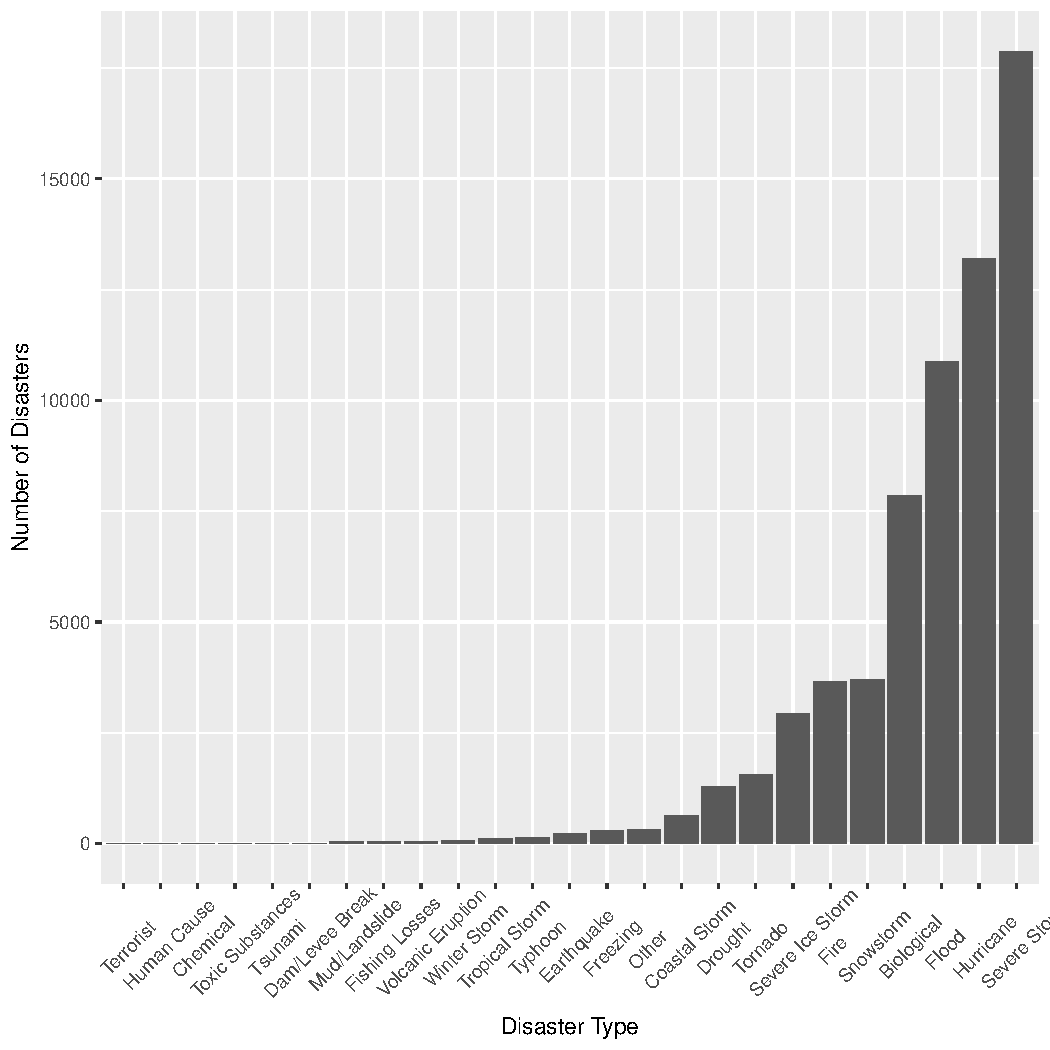
\includegraphics[width=\maxwidth]{figure/histogram_disasters-1} 
\end{knitrout}

  \caption{Histogram of the total number of disasters declared by the United States} 
  \label{figure:1}
  \end{minipage}
\end{figure}

\clearpage
\begin{knitrout}
\definecolor{shadecolor}{rgb}{0.969, 0.969, 0.969}\color{fgcolor}\begin{kframe}
\begin{verbatim}
##       1       2       3       4       5       6       7       8 
## 1654.88 1680.01 1705.14 1730.27 1755.40 1780.53 1805.66 1830.79 
##       9      10      11      12 
## 1855.92 1881.05 1906.18 1931.32
## 
## Call:
## lm(formula = DisasterCount ~ Year, data = annual_disasters)
## 
## Residuals:
##     Min      1Q  Median      3Q     Max 
## -714.57 -312.30  -49.99  177.93 1361.83 
## 
## Coefficients:
##               Estimate Std. Error t value Pr(>|t|)    
## (Intercept) -49209.962   4821.925  -10.21 2.80e-15 ***
## Year            25.131      2.426   10.36 1.51e-15 ***
## ---
## Signif. codes:  0 '***' 0.001 '**' 0.01 '*' 0.05 '.' 0.1 ' ' 1
## 
## Residual standard error: 409.4 on 67 degrees of freedom
## Multiple R-squared:  0.6156,	Adjusted R-squared:  0.6098 
## F-statistic: 107.3 on 1 and 67 DF,  p-value: 1.514e-15
\end{verbatim}
\end{kframe}
\end{knitrout}

\begin{figure}[h!]
\centering
  \begin{minipage}{.8\linewidth}
\begin{knitrout}
\definecolor{shadecolor}{rgb}{0.969, 0.969, 0.969}\color{fgcolor}
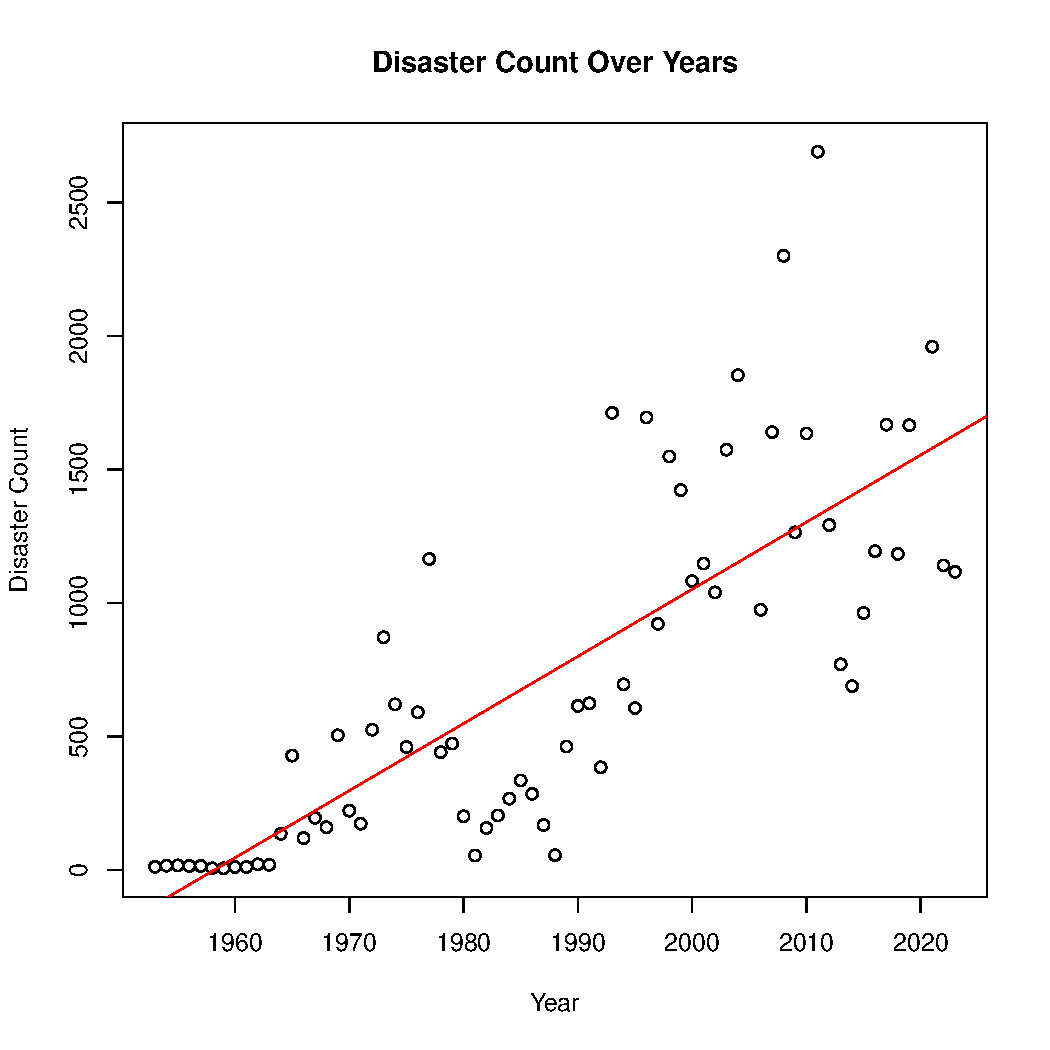
\includegraphics[width=\maxwidth]{figure/plot_data_points-1} 
\end{knitrout}
  \label{figure:2}
  \end{minipage}
\end{figure}

\section*{Model Summary}
The summary of the linear model offers key insights:
\subsection*{Coefficients:}
\begin{itemize}
    \item The intercept is $-49209.962$, implying the model's prediction for \textit{DisasterCount} when \textit{Year} is 0, which is not applicable in this context.
    \item The slope coefficient for \textit{Year} is $25.131$. This indicates an annual increase of approximately 25.131 in \textit{DisasterCount}, as per the model.
    \item These predictions indicate an upward trend in \textit{DisasterCount} over the years.
\end{itemize}
\subsection*{Statistical Significance:}
\begin{itemize}
  \item Both the intercept and the slope demonstrate statistical significance with a p-value $< 0.001$.
\end{itemize}
\subsection*{Model Fit:}
\begin{itemize}
    \item The R-squared value is $0.6156$, signifying that approximately 61.56\% of the variability in \textit{DisasterCount} is explained by the year. However, a significant portion of variability remains unexplained.
    \item The Residual Standard Error (RSE) is $409.4$, indicating the average deviation of data points from the fitted line.
\end{itemize}
\subsection*{Residuals:}
\begin{itemize}
  \item The residuals range from $-714.57$ to $1361.83$, suggesting variability around the regression line.
\end{itemize}
\section*{Interpretation and Considerations}
\begin{itemize}
    \item The Biological factor and the years 2020, 2005, and 2024 where filtered out of linear model
    \item The model indicates a significant upward trend in disaster counts over the years.
    \item The presence of significant residuals and a R-squared value of $0.6156$ implies that, while there is a discernible trend, other unaccounted factors might also be influencing \textit{DisasterCount}.
    \item Predictions for future years should be approached with caution due to the simplicity of the model and its exclusion of other potential predictive factors.
    \item When interpreting these results and making future decisions, the limitations of a simple linear regression model and the impact of external factors not included in the model should be considered.
    \item Severe Storms, Hurricanes, Floods, and Biological make up the majority of declared disasters.
    \item Further analysis of the top 3 populated factors present in the Histogram should be considered.
\end{itemize}
\end{document}
